\documentclass[11pt,psfig]{article}
\usepackage{epsfig}
\usepackage{times}
\usepackage{amssymb}
\usepackage{float}

\newcount\refno\refno=1
\def\ref{\the\refno \global\advance\refno by 1}
\def\ux{\underline{x}}
\def\uw{\underline{w}}
\def\bw{\underline{w}}
\def\ut{\underline{\theta}}
\def\umu{\underline{\mu}} 
\def\bmu{\underline{\mu}} 
\def\be{p_e^*}
\newcount\eqnumber\eqnumber=1
\def\eq{\the \eqnumber \global\advance\eqnumber by 1}
\def\eqs{\eq}
\def\eqn{\eqno(\eq)}

 \pagestyle{empty}
\def\baselinestretch{1.1}
\topmargin1in \headsep0.3in
\topmargin0in \oddsidemargin0in \textwidth6.5in \textheight8.5in
\begin{document}
\setlength{\parskip}{1.2ex plus0.3ex minus 0.3ex}


\thispagestyle{empty} \pagestyle{myheadings} \markright{Homework
\#: CS 216, Image Understanding: Spring 2014}



\title{CS 216 Homework 2}
\author{Zachary DeStefano, 15247592}
\date{Due Date: April 25, 2014}

\maketitle

\vfill\eject

\newpage

\section*{Problem 1}

We will prove that $(f*g)*h=f*(g*h)$. First off, let $x=f*g$ and let $y=g*h$. \\
\[
x(t) = (f*g)(t) = \sum_{s=-\infty}^{\infty} f(t-s)g(s)
\]
\[
y(t) = (g*h)(t) = \sum_{s=-\infty}^{\infty} g(s)h(t-s)
\]
This means that
\[
(x*h)(t) = \sum_{v=-\infty}^{\infty} x(v)h(t-v) = \sum_{v=-\infty}^{\infty} \sum_{s=-\infty}^{\infty} f(v-s)g(s)h(t-v)
\]
Similarly
\[
(f*y)(t) = \sum_{v=-\infty}^{\infty} f(t-v)y(v) = \sum_{v=-\infty}^{\infty} \sum_{s=-\infty}^{\infty} f(t-v)g(s)h(v-s)
\]
In the second equation, do a change of variables $v = t-v'+s$ which does not change the final result since we are going from negative infinity to infinity. For the second equation, we end up with \\
\[
(f*y)(t) = \sum_{v'=-\infty}^{\infty} \sum_{s=-\infty}^{\infty} f(v'-s)g(s)h(t-v')
\]
As can be observed, the first and second equation are now equal. This proves that $(x*h)(t)=(f*y)(t)$ and since this applies for any three functions, we have proven that convolution is associative. 

\newpage

\section*{Problem 2}

If we correlate a function $f$ with an impulse function, we get $f(-t)$, \\
so the function gets flipped around the y-axis. \\
Here is the proof:\\
Take the impulse function g, so $g(0)=1$ and $g(x)=0$ for all other $x$ \\
Let * be the correlation operation in this case. \\
\[
(f*g)(t) = \sum_{s=-\infty}^{\infty} f(s)g(s+t)
\]
In our case, the inner term is always $0$ except for when $s+t=0$ so $s=-t$, \\
thus $(f*g)(t)=f(-t)$, proving our assertion. \\
\\
Now let $h(t)=g(t)$. We will prove that $(f*g)*h \neq f*(g*h)$. \\
\\
For the right hand side, by what was shown above, \\
$g*h = g$ since the impulse function is symmetric around the y-axis. \\
This means that $(f*(g*h))(t) = (f*g)(t) = f(-t)$. \\
\\
For the left hand side, by what was shown above, \\
$(f*g)(t) = f(-t)$ thus $((f*g)*h)(t) = (f(-t))*h(t)$\\
This will flip the function back to its original position, thus the left hand side is equal to $f(t)$\\
\\
For any non-symmetric function $f$, such as $f(t) = 3t+5$, it holds that $f(t) \neq f(-t)$ \\
thus the left hand side is not equal to the right hand side. \\
\\
Since we have example functions whose correlations are not associative, there is no way correlation is associative. 

\newpage

\section*{Problem 3}

Let $g_1(x) = g_2(y) = N(0,\sigma^2)$. Then
\[
g_1(x) = \frac{1}{\sqrt{2\pi \sigma^2}} e^{-\frac{x^2}{2\sigma^2}}
\]
\[
g_2(y) = \frac{1}{\sqrt{2\pi \sigma^2}} e^{-\frac{y^2}{2\sigma^2}}
\]
This means that
\[
g_1(x)g_2(y) = \frac{1}{2\pi \sigma^2} e^{-\frac{x^2 + y^2}{2\sigma^2}}
\]
This is equal to $g(x,y)$, thus allowing us to say that $g(x,y) = g_1(x)g_2(y)$

\newpage

\section*{Problem 4}

For the spatial domain running time, we can think of convolution as the following:\\
- For each pixel in the image, we apply the filter to it. \\
Thus there are $H \cdot W$ iterations of the filter\\
Each filter will take $M \cdot N$ time. \\
Thus the time complexity is $O(MNHW)$\\
\\
If we use FFT, this would be the procedure:\\
1. Convert the signal to frequency\\
2. Convert the filter to frequency \\
3. Do element wise multiplication of the two new vectors. \\
4. Convert the elements back. \\
\\
Step 1 will take $MN \cdot log(MN)$ time\\
Step 2 will take $HW \cdot log(HW)$ time\\
Step 3 will take $max(HW,MN)$ time. The identity of the max will not matter in the end since the previous step eclipses this one. \\
Step 4 will take $max(HW,MN) log( max(HW, MN) )$ time. Again which one is the max does not matter because of step 1 and 2. \\
\\
The total running time is thus $O(MN \cdot log(MN) + HW \cdot log(HW) )$ in the case where we use FFT. \\
Assuming that $HW$ is the max, the running time is $O(HW \cdot log(HW))$. \\
\\
If the filter is $f(x,y) = f_1(x)f_2(y)$, then assuming that $I$ is the image, it holds that $I*f = (I*f_1)*f_2$\\
Here is the proof:\\
\[
(f*I)(x,y) = \sum_{i=-\infty}^{\infty} \sum_{j=-\infty}^{\infty} f(i,j)I(x-i,y-j)
\]
By separability,
\[
(f*I)(x,y) = \sum_{i=-\infty}^{\infty} \sum_{j=-\infty}^{\infty} f_1(i)f_2(j)I(x-i,y-j)
\]
\[
(f*I)(x,y) = \sum_{i=-\infty}^{\infty} f_1(i) (\sum_{j=-\infty}^{\infty} f_2(j)I(x-i,y-j))
\]
The inner summation is just convolution, thus we have
\[
(f*I)(x,y) = \sum_{i=-\infty}^{\infty} f_1(i) (I*f_2)(i)
\]
The summation shown here is convolution again, thus
\[
(f*I)(x,y) = (I*f_2)*f_1
\]
By associativity and commutativity of convolution, $f*I=(I*f_1)*f_2$, proving our assertion. \\
\\
By what was just shown, we can do this procedure:\\
1. Convolve the image horizontally. \\
2. Convolve the result vertically. \\
Step 1 will take $O(HWM)$ time and step 2 will take $O(HWN)$ time, \\
thus the total running time is $O(HW \cdot max(M,N))$. \\
Assuming $M$ is the max, the running time is $O(HWM)$.\\
Thus, by doing the horizontal filter then vertical filter, we can do even better than if we convert to frequency space. \\ 

\newpage

\section*{Problem 5}

Our two gaussians are as follows
\[
g_1(t) = \frac{1}{\sqrt{2\pi \sigma_1^2}} e^{-\frac{t^2}{2\sigma_1^2}}
\]
\[
g_2(t) = \frac{1}{\sqrt{2\pi \sigma_2^2}} e^{-\frac{t^2}{2\sigma_2^2}}
\]
The convolution formula we will use is the following
\[
g_3(t) = \int_{-\infty}^{\infty}{g_1(s)g_2(t-s) \, ds}
\]
Let $F_1$ be the Fourier transform for $g_1$ and $F_2$ be the transform for $g_2$.\\
\[
F_1(t) = \int_{-\infty}^{\infty}{g_1(s) e^{-2\pi i s t} \, ds}
\]
\[
F_2(t) = \int_{-\infty}^{\infty}{g_2(s) e^{-2\pi i s t} \, ds}
\]
Expanding we have
\[
F_1(t) = \frac{1}{\sqrt{2 \pi \sigma_1^2}} \int_{-\infty}^{\infty}{e^{-\frac{s^2}{2\sigma_1^2}} e^{-2\pi i s t} \, ds}
\]
\[
F_2(t) = \frac{1}{\sqrt{2 \pi \sigma_2^2}} \int_{-\infty}^{\infty}{e^{-\frac{s^2}{2\sigma_2^2}} e^{-2\pi i s t} \, ds}
\]
Using Euler's Formula we can now say that
\[
F_1(t) = \frac{1}{\sqrt{2 \pi \sigma_1^2}} \int_{-\infty}^{\infty}{e^{-\frac{s^2}{2\sigma_1^2}} (cos(2\pi s t) + i sin(2\pi s t)) \, ds}
\]
\[
F_2(t) = \frac{1}{\sqrt{2 \pi \sigma_2^2}} \int_{-\infty}^{\infty}{e^{-\frac{s^2}{2\sigma_2^2}} (cos(2\pi s t) + i sin(2\pi s t)) \, ds}
\]
Since the sine is an odd function, the integral of it will go to zero, thus we can simplify the above equations
\[
F_1(t) = \frac{1}{\sqrt{2 \pi \sigma_1^2}} \int_{-\infty}^{\infty}{e^{-\frac{s^2}{2\sigma_1^2}} cos(2\pi s t) \, ds}
\]
\[
F_2(t) = \frac{1}{\sqrt{2 \pi \sigma_2^2}} \int_{-\infty}^{\infty}{e^{-\frac{s^2}{2\sigma_2^2}} cos(2\pi s t) \, ds}
\]
This Wolfram Alpha web page explains the result of that integration. 
\begin{verbatim}
http://mathworld.wolfram.com/FourierTransformGaussian.html
\end{verbatim}
We can now use that fact to assert that
\[
F_1(t) = \frac{1}{\sqrt{2 \pi \sigma_1^2}} \sqrt{2 \pi \sigma_1^2} \, e^{-2 \pi^2 t^2 \sigma_1^2}
\]
\[
F_2(t) = \frac{1}{\sqrt{2 \pi \sigma_2^2}} \sqrt{2 \pi \sigma_2^2} \, e^{-2 \pi^2 t^2 \sigma_2^2}
\]
Simplifying we have the following
\[
F_1(t) = e^{-2 \pi^2 t^2 \sigma_1^2}
\]
\[
F_2(t) = e^{-2 \pi^2 t^2 \sigma_2^2}
\]
Let $F=F_1 \cdot F_2$ since we want to multiply the frequency functions, then we have
\[
F(t) = e^{-2 \pi^2 t^2 (\sigma_1^2 + \sigma_2^2)}
\]
Let $\sigma = -2 \pi^2 (\sigma_1^2 + \sigma_2^2)$, then 
\[
F(t) = e^{\sigma t^2}
\]
We want the inverse transform of $F$ to get the convolution. Thus we can say that 
\[
g_3(x) = \int_{-\infty}^{\infty} e^{2\pi i x t} F(t) dt
\]
\[
g_3(x) = \int_{-\infty}^{\infty} e^{2\pi i x t}e^{\sigma t^2} dt
\]
Expanding using Euler's formula and using the fact that sine is an odd function, we can say that
\[
g_3(x) = \int_{-\infty}^{\infty} cos(2 \pi x t)e^{\sigma t^2} dt
\]
This is the same integral as was in the Wolfram Alpha web page, thus we can assert that
\[
g_3(x) = \sqrt{-\frac{\pi}{\sigma}} \, e^{\frac{\pi^2 x^2}{\sigma}}
\]
Expanding $\sigma$ and then simplifying, we have
\[
g_3(x) = \frac{1}{\sqrt{2\pi (\sigma_1^2 + \sigma_2^2)}} \, e^{-\frac{x^2}{2(\sigma_1^2 + \sigma_2^2)}}
\]
If we let $\sigma_3 = \sqrt{\sigma_1^2 + \sigma_2^2}$ then we have
\[
g_3(x) = \frac{1}{\sqrt{2\pi \sigma_3^2}} \, e^{-\frac{x^2}{2\sigma_3^2}}
\]
This is clearly a Gaussian with variance $\sigma_3$ as defined above, thus $g_3$ is a Gaussian as desired.\\
\newpage
We can use this formula instead of normal convolution formula to find the convolution of two Gaussians and it will save us computation time. \\
\\
Assuming that we have two Gaussian filters of size $M \times N$ that we want to convolve,
using the normal formula, the convolution of them will take $O(M^2 N^2)$ time. \\
\\
From what was shown above we already have the formula,
thus we can apply it to each slot in the filter making the time complexity $O(MN)$. \\

\newpage

\section*{Problem 6}

\subsection*{Initial 1D Plots}

\begin{figure}[H]
\centering
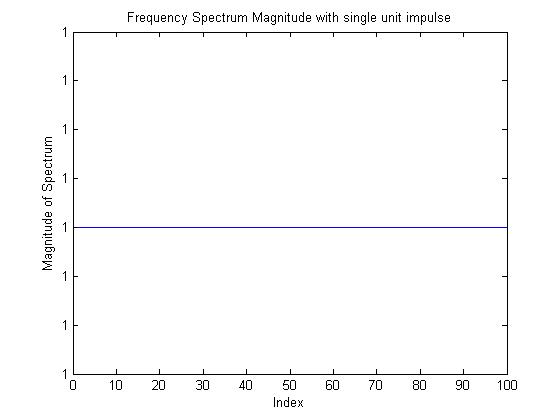
\includegraphics[height=3in]{prob6plot_freq1.jpg}
\caption{Frequency Spectrum Magnitude Plot for single impulse}
\end{figure}

\begin{figure}[H]
\centering
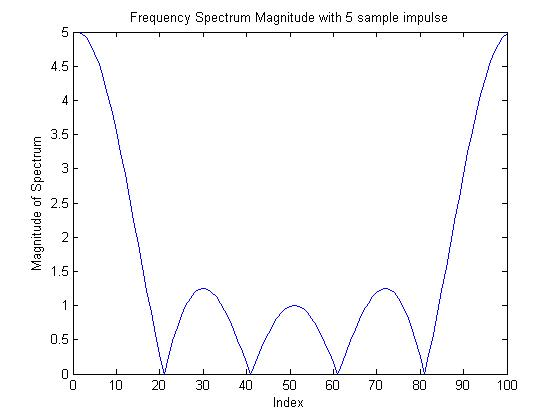
\includegraphics[height=3in]{prob6plot_freq5.jpg}
\caption{Frequency Spectrum Magnitude Plot for 5 sample impulse}
\end{figure}

\begin{figure}[H]
\centering
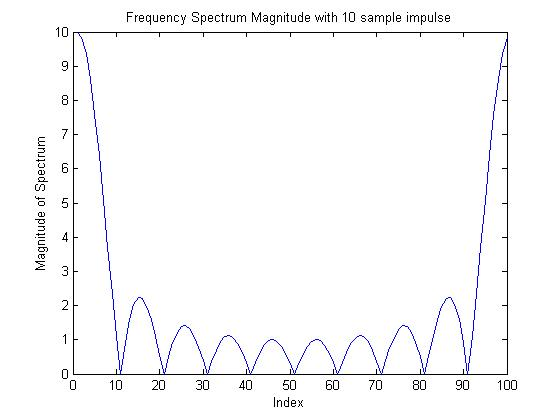
\includegraphics[height=3in]{prob6plot_freq10.jpg}
\caption{Frequency Spectrum Magnitude Plot for 10 sample impulse}
\end{figure}

\begin{figure}[H]
\centering
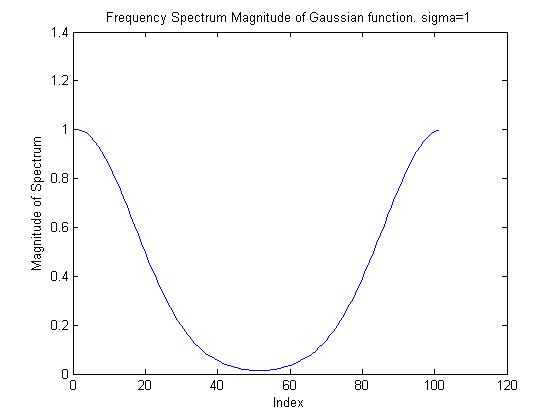
\includegraphics[height=3in]{prob6plot_freqGauss1.jpg}
\caption{Frequency Spectrum Magnitude Plot for Gaussian Function with $\sigma=1$}
\end{figure}

\begin{figure}[H]
\centering
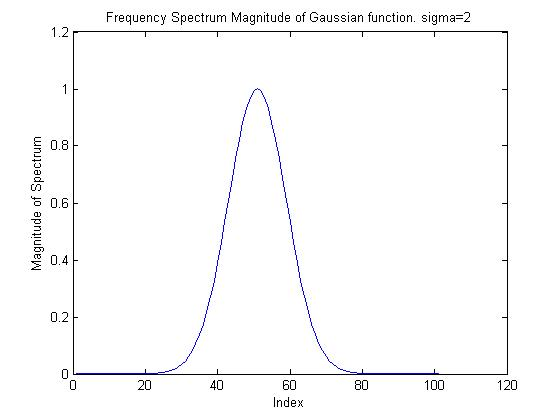
\includegraphics[height=3in]{prob6plot_freqGauss2.jpg}
\caption{Frequency Spectrum Magnitude Plot for Gaussian Function with $\sigma=2$}
\end{figure}

\subsection*{Magnitude and Phase Experiment for Zebra and Simpsons}

\begin{figure}[H]
\centering
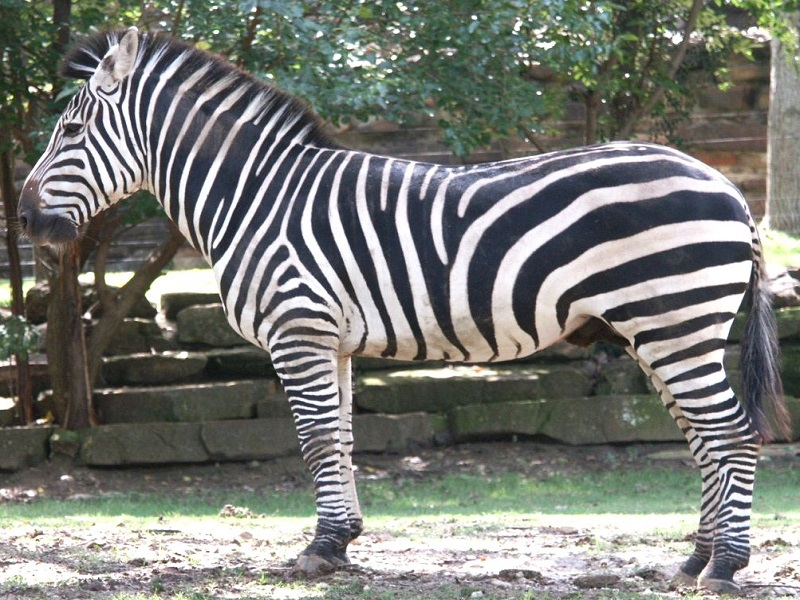
\includegraphics[height=3in]{zebraMod.jpg}
\caption{The Zebra picture, modified to be the same size as the simpsons picture}
\end{figure}

\begin{figure}[H]
\centering
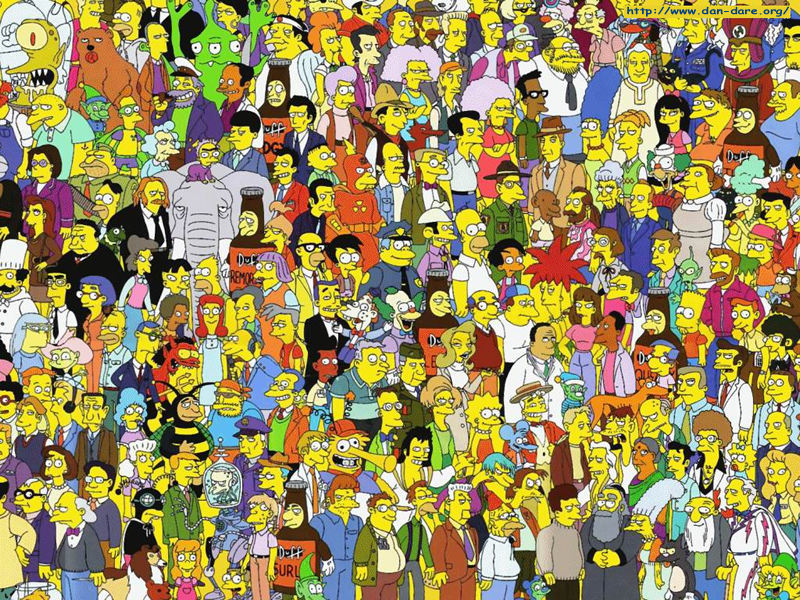
\includegraphics[height=3in]{simpsons.jpg}
\caption{The Simpsons picture}
\end{figure}

\begin{figure}[H]
\centering
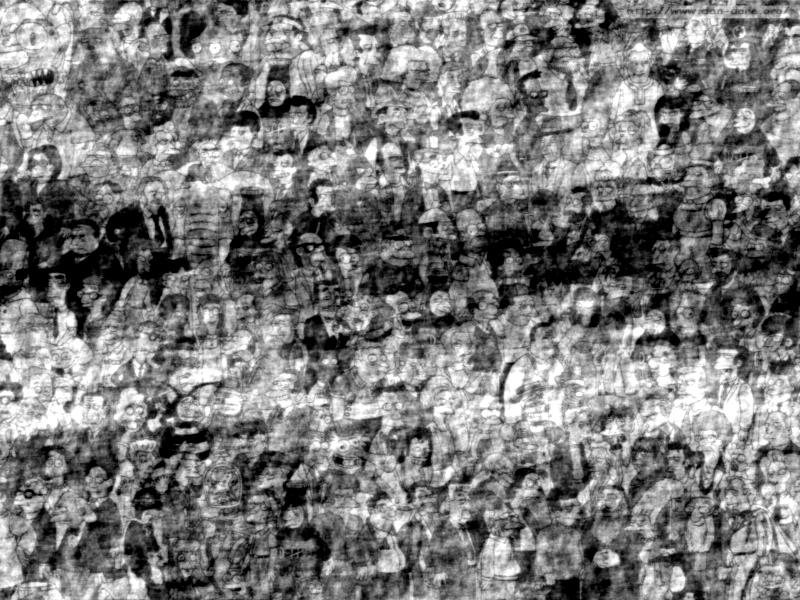
\includegraphics[height=3in]{mag_zebra_phase_simpsons.jpg}
\caption{Magnitude of Zebra picture with Phase of Simpsons picture}
\end{figure}

\begin{figure}[H]
\centering
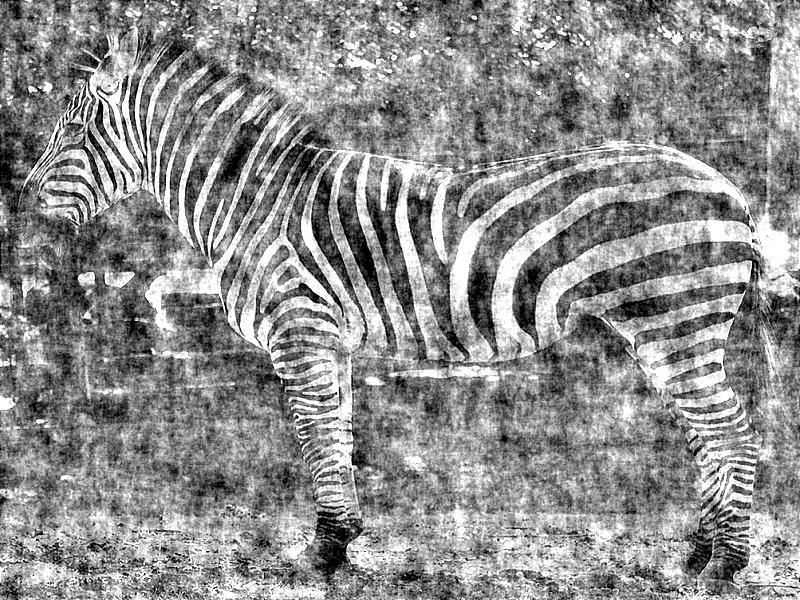
\includegraphics[height=3in]{mag_simpsons_phase_zebra.jpg}
\caption{Magnitude of Simpsons picture with Phase of Zebra picture}
\end{figure}

\subsection*{Other Interesting Result}

\begin{figure}[H]
\centering
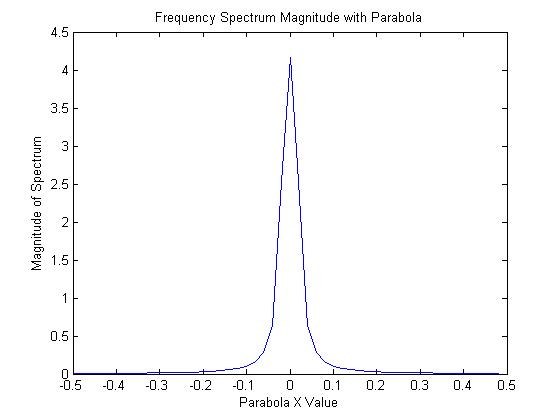
\includegraphics[height=3in]{prob6plot_freqParabola.jpg}
\caption{Frequency Spectrum Magnitude Plot for the Parabola $y=x^2$}
\end{figure}

I plotted the frequency spectrum for a parabola and found the result interesting. The frequency spectrum magnitude seems to tend toward infinity as we approach the vertex and tends toward zero away from the vertex in both directions.\\
\newpage 

\section*{Problem 7}

\subsection*{Pictures for Zebra Image where $\sigma=2$}

\begin{figure}[H]
\centering
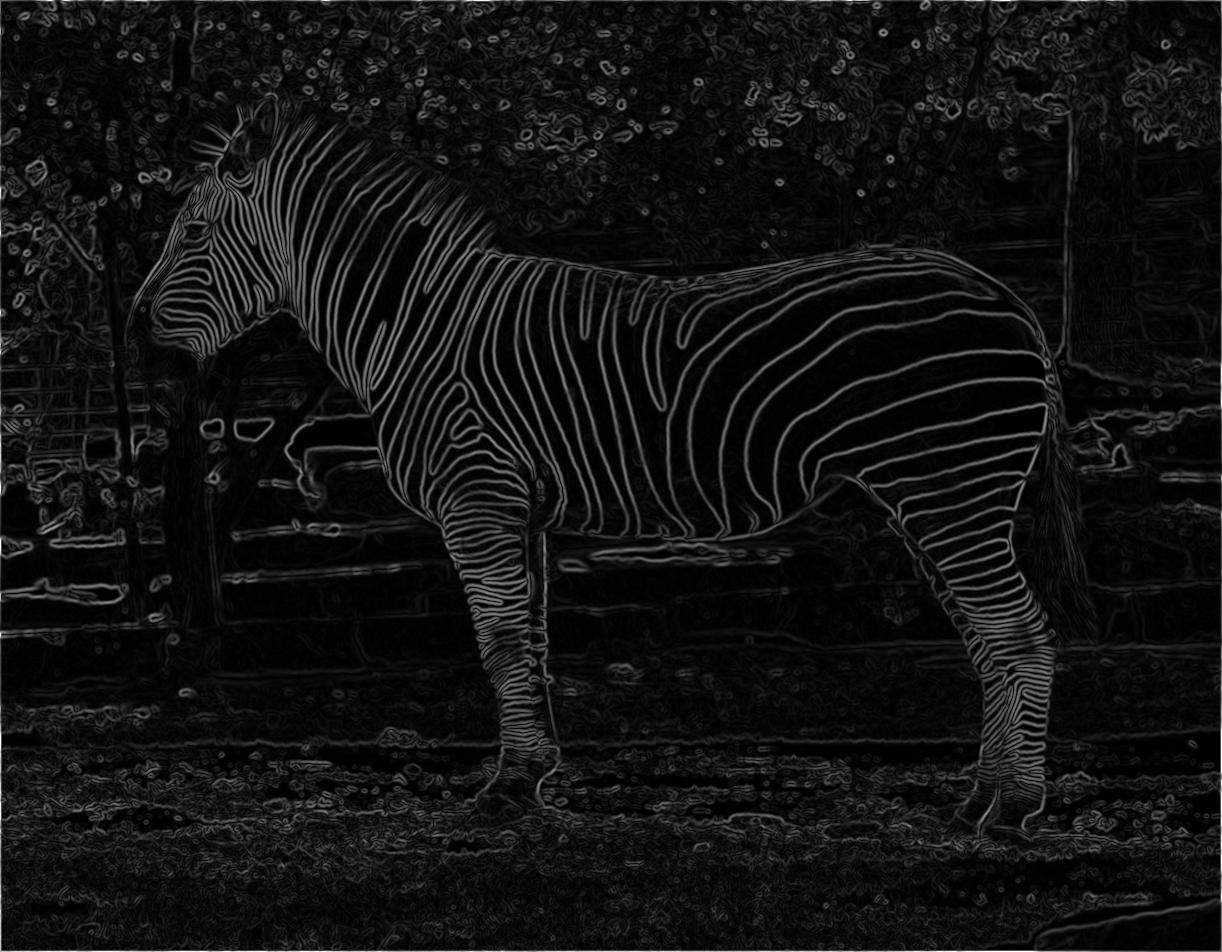
\includegraphics[height=3in]{magGradient_zebra1.jpg}
\caption{Magnitude of the Gradient of the zebra picture where $\sigma=2$}
\end{figure}

\begin{figure}[H]
\centering
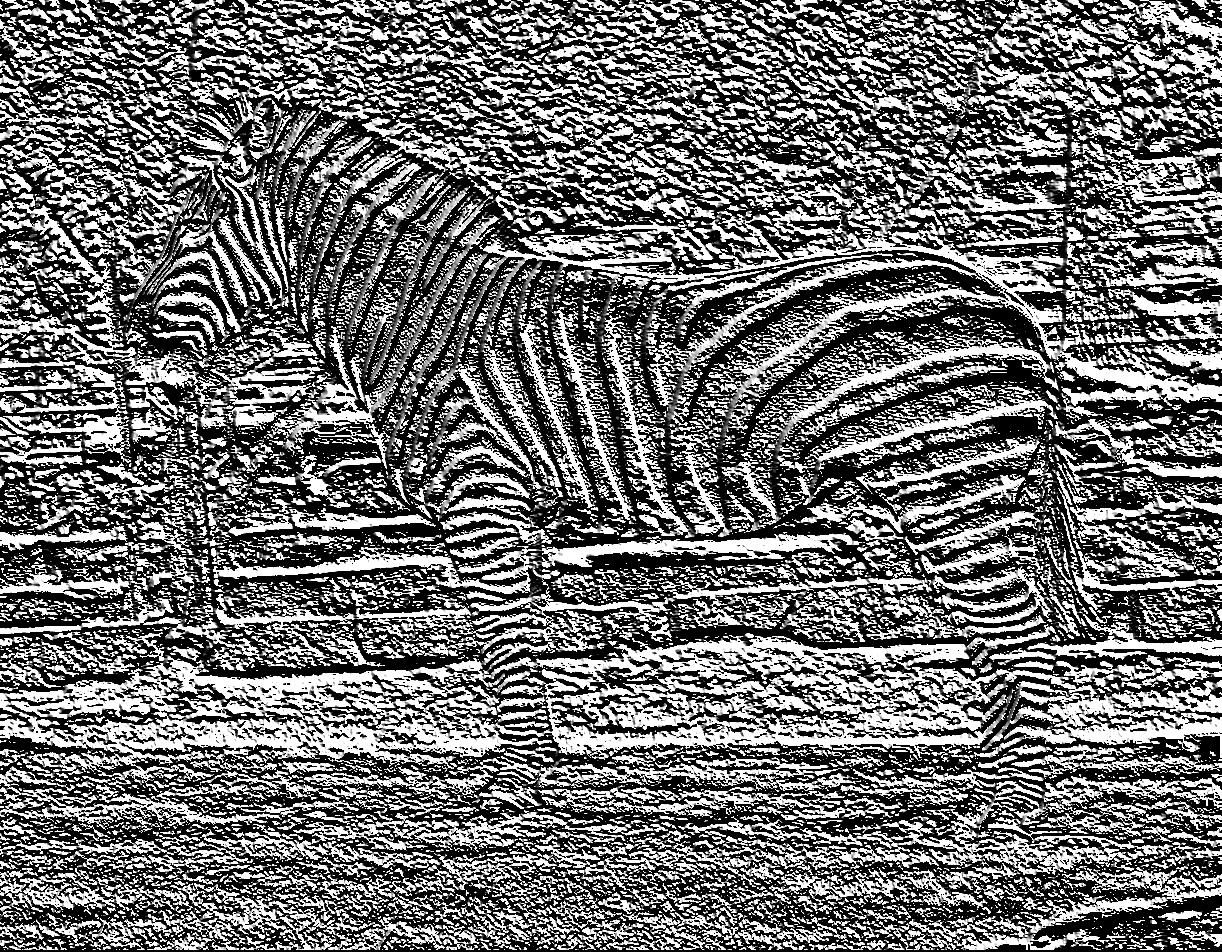
\includegraphics[height=3in]{orientGradient_zebra1.jpg}
\caption{Orientation of the Gradient of the zebra picture where $\sigma=2$}
\end{figure}

\subsection*{Pictures for Zebra Image where $\sigma=3$}

\begin{figure}[H]
\centering
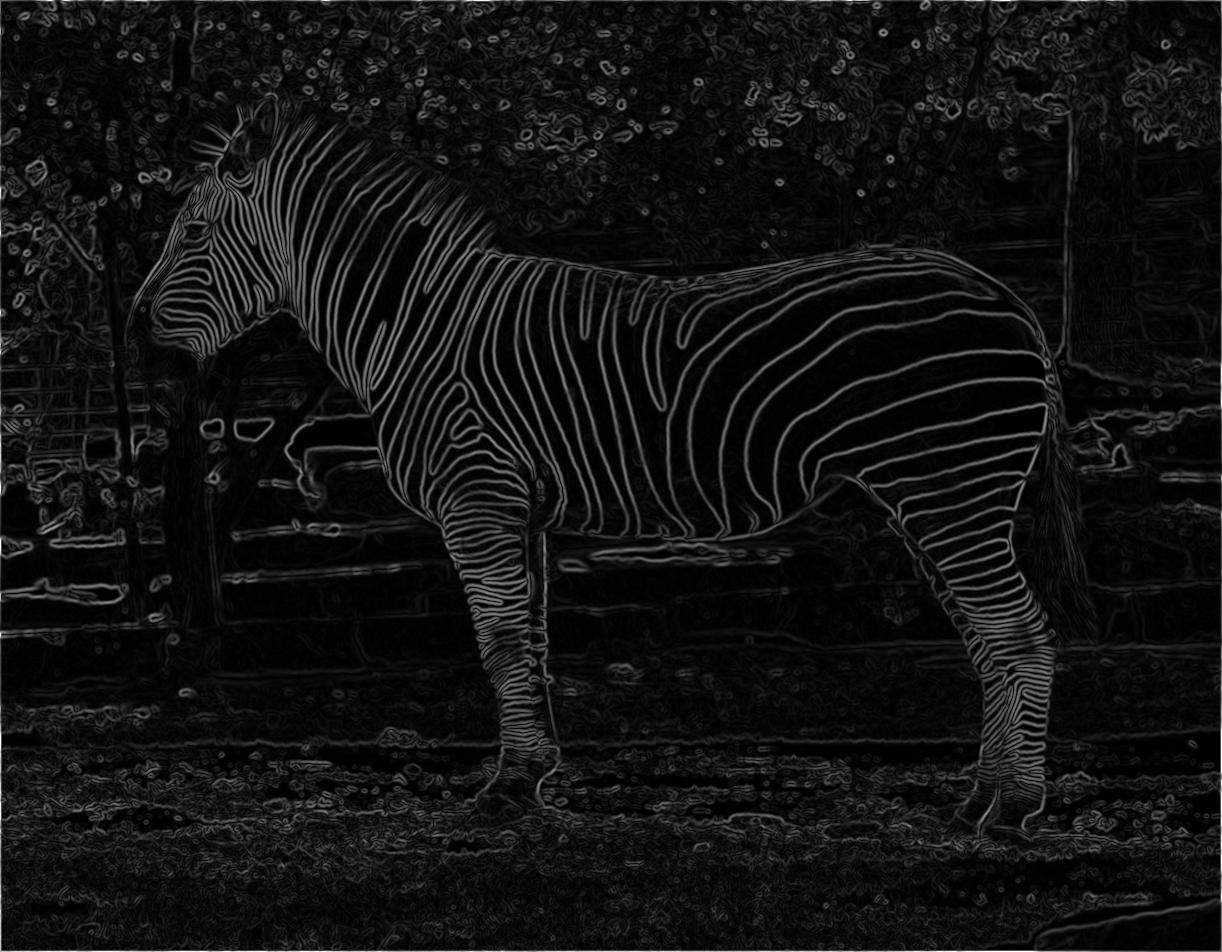
\includegraphics[height=3in]{magGradient_zebra1.jpg}
\caption{Magnitude of the Gradient of the zebra picture where $\sigma=3$}
\end{figure}

\begin{figure}[H]
\centering
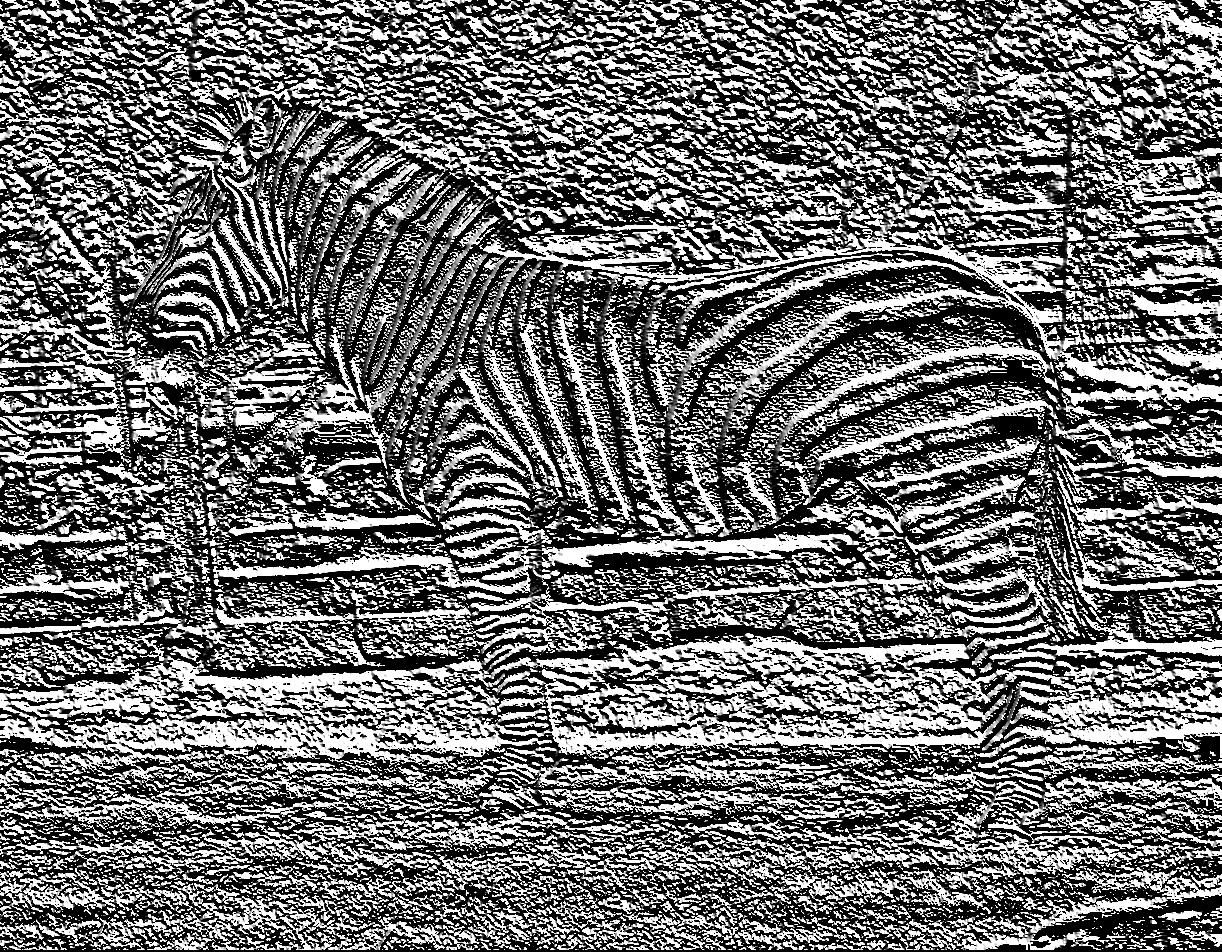
\includegraphics[height=3in]{orientGradient_zebra1.jpg}
\caption{Orientation of the Gradient of the zebra picture where $\sigma=3$}
\end{figure}

\newpage

\subsection*{Matlab code}

\begin{verbatim}
picname = 'zebra1.jpg'; %specify which pic to use
imageData = im2double(rgb2gray(imread(picname)));
figure
imagesc(imageData);
colorbar
title('Original Image');

sigma = 3; %change this to sigma=2 for other example
gaussFilt = fspecial('gaussian',sigma);
filteredImageData = conv2(imageData,gaussFilt,'same');
figure
imagesc(filteredImageData);
colorbar
title('Filtered Image');

horizDerivFilter = [1 -1];
horizDerivImage = conv2(filteredImageData,horizDerivFilter,'same');
figure
imagesc(horizDerivImage);
colorbar;
title('Horizontal Derivative Image');

vertDerivFilter = transpose(horizDerivFilter);
vertDerivImage = conv2(filteredImageData,vertDerivFilter,'same');
figure
imagesc(vertDerivImage);
colorbar;
title('Vertical Derivative Image');

complexDerivImage = horizDerivImage + vertDerivImage.*1i;

figure
magDerivImage = abs(complexDerivImage);
imagesc(magDerivImage);
imwrite(magDerivImage,strcat('magGradient2_',picname),'JPEG');
colorbar;
title('Magnitude of the Gradient');

figure
orientationDerivImage = angle(complexDerivImage);
imagesc(orientationDerivImage);
imwrite(orientationDerivImage,strcat('orientGradient2_',picname),'JPEG');
colorbar;
title('Orientation of the Gradient');
\end{verbatim}

\newpage

\section*{Problem 8}

I worked with the dilbert cartoon and attempted to detect the letter N. Before I did anything, I inverted the image, so that all the stuff we care about has value $1$ and the background that we do not care about has value $0$. 

\subsection*{Object Detection Results}

\begin{figure}[H]
\centering
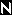
\includegraphics[height=1in]{template_dilbert1.jpg}
\caption{The template used for the letter N}
\end{figure}

\begin{figure}[H]
\centering
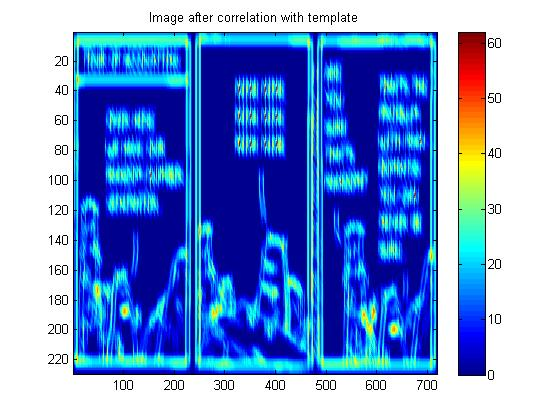
\includegraphics[height=4in]{prob8plot_afterCorrelation.jpg}
\caption{Plot after doing correlation of the dilbert image with the template}
\end{figure}

\begin{figure}[H]
\centering
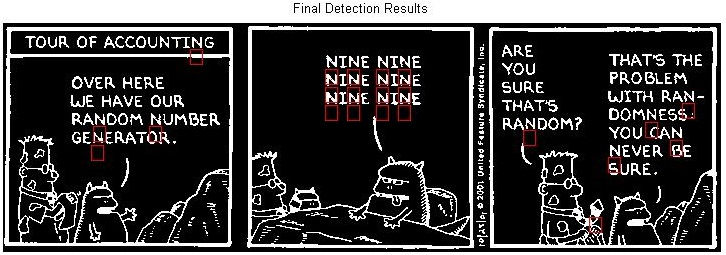
\includegraphics[height=2.5in]{prob8plot_finalDetection.jpg}
\caption{Final Detection Results}
\end{figure}

\subsection*{Matlab code}

\begin{verbatim}
imageName = 'dilbert1.jpg';

%for dilbert, it is already BW, so no need to call rgb2gray
rawImageData = 1-im2double(imread(imageName));
imageData = double((rawImageData > 0.5));

%figure
%imshow(imageData)

%used to get the corner values of the square we care about 
%[xVals,yVals] = ginput(2)

%values for the word "Nine"
rightX = 386;
leftX = 375;
bottomY = 50;
topY = 64;

nLetterImageData = imageData(bottomY:topY,leftX:rightX);
imwrite(nLetterImageData,'template_dilbert1.jpg','JPEG');

%correlation = xcorr2(imageData,nLetterImageData);
%correlation = xcorr2(nLetterImageData,imageData);
Template = flipud(fliplr(nLetterImageData));
correlation = conv2(imageData,Template,'same');
figure
imagesc(correlation);
colorbar;
title('Image after correlation with template');

%does the thresholding
%this is the 1-D example. It needs to be extended to 2D
%threshold = mean(correlation(:)); %this is currently 387
threshold = 47;
L = (correlation(2:end-1,2:end-1) > correlation(1:end-2,2:end-1));
R = (correlation(2:end-1,2:end-1) > correlation(3:end,2:end-1));

%upper left, right, and middle ones
UL = (correlation(2:end-1,2:end-1) > correlation(1:end-2,1:end-2));
UM = (correlation(2:end-1,2:end-1) > correlation(2:end-1,1:end-2));
UR = (correlation(2:end-1,2:end-1) > correlation(3:end,1:end-2));

%lower left, right, and middle ones
LL = (correlation(2:end-1,2:end-1) > correlation(1:end-2,3:end));
LM = (correlation(2:end-1,2:end-1) > correlation(2:end-1,3:end));
LR = (correlation(2:end-1,2:end-1) > correlation(3:end,3:end));

T = (correlation(2:end-1,2:end-1) > threshold);
maxima = R & L & T & UL & UM & UR & LL & LM & LR;

%preps data for the overlay
%  for the grayscale to rgb, all the color channels are the same
imageDataSize = size(imageData);
rgbImageData = zeros(imageDataSize(1),imageDataSize(2),3);
rgbImageData(:,:,1) = imageData;
rgbImageData(:,:,2) = imageData;
rgbImageData(:,:,3) = imageData;
maximaInverted = 1-maxima;

%puts red dots at the maxima points
%  this is done by zeroing each channel at a maxima point
%  For the red channel, zeros are put at the maxima points 
%       and then a 1 value is put there
rgbImageData(2:end-1,2:end-1,1) = imageData(2:end-1,2:end-1).*maximaInverted + maxima;
rgbImageData(2:end-1,2:end-1,2) = imageData(2:end-1,2:end-1).*maximaInverted;
rgbImageData(2:end-1,2:end-1,3) = imageData(2:end-1,2:end-1).*maximaInverted;

figure
imshow(rgbImageData);
title('Final Detection Results');
sizeMaxima = size(maxima);
sizeTemplate = size(Template);
horizSizeTemplate = sizeTemplate(2);
vertSizeTemplate = sizeTemplate(1);
for y = 1:sizeMaxima(1)
   for x = 1:sizeMaxima(2)
      if(maxima(y,x) > 0)
          xCoord = (x+1) - horizSizeTemplate/2;
          yCoord = (y+1) + vertSizeTemplate/2;
         rectangle('Position',[xCoord yCoord horizSizeTemplate vertSizeTemplate],'LineWidth',1,'EdgeColor','r');
      end
   end
end

\end{verbatim}

\newpage

\section*{Problem 9}

In this case, trying to use the sum of squared differences did not help. The best option was using the correlation template as was done in problem 8. I used the same image and template for the object I wanted to detect and no matter what variance threshold was used, the N letters were not detected and other things were detected instead. Here is the final detection result when using sum of squared differences and the best variance threshold. 

\begin{figure}[H]
\centering
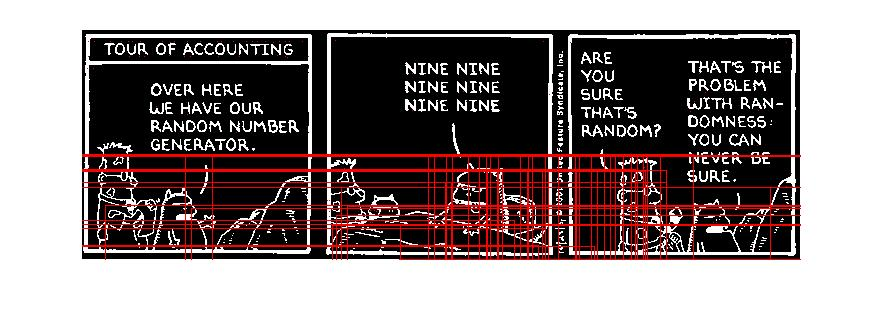
\includegraphics[height=2.5in]{prob9plot_finalDetection.jpg}
\caption{Final Detection Results, threshold is 104}
\end{figure}

\end{document}








